\hypertarget{iab}{%
\chapter{Institute for Employment Research, Germany: Access to Administrative Labor Market Data for International Researchers}\label{iab}}

\printchapterauthor{%
\begin{authorlist}
  Dana Müller (Institute for Employment Research)  \\
  Philipp vom Berge (Institute for Employment Research)  \\
\end{authorlist}}\authorfootnote{Müller, Dana,  and Philipp vom Berge}{Dana Müller and Philipp vom Berge}{iab}
\authortoc{Dana Müller, Philipp vom Berge}
\hrulefill

\hypertarget{summary-1}{%
\section{Summary}\label{summary-1}}

This chapter describes the Research-Data-Center in Research-Data-Center\index{Research-Data-Center in Research-Data-Center} RDC-in-RDC\index{Research-Data-Center in Research-Data-Center} approach, which is a project that implemented decentralized data access to confidential German labor market data provided by the Research Data Center at the Institute for Employment Research\index{Research Data Center at the Institute for Employment Research} RDC-IAB in Nuremberg, Germany via data access points\index{data access points} at collaborating research data centers\index{Research Data Center} (RDC), research institutes, and universities. RDC-in-RDC improves data access for researchers who want to work with confidential data but are unable to come to Nuremberg to work with the data on-site\index{On-site}. The project started in 2010 and was funded by the German Federal Ministry of Education and Research\index{German Federal Ministry of Education and Research} (BMBF). The chapter covers the challenges involved in developing standardized procedures in an international context in order to ensure user-friendly and sustainable data access in compliance with legal requirements.

The RDC-IAB\index{Research Data Center at the Institute for Employment Research}, founded in 2004, is a research department of the Institute for Employment Research\index{Institute for Employment Research} (IAB), which belongs to the Federal Employment Agency\index{Federal Employment Agency} (BA) of Germany. The RDC-IAB has three core functions: creating standardized research data for the scientific community, providing access to these data, and conducting research with and about IAB data. Various kinds of standardized labor market data are provided by the RDC-IAB. Administrative research data are based on the notification procedure of the German Social Security System and process-generated data are based on the BA. Additionally, surveys conducted by the IAB or partner institutes become part of the data portfolio. Furthermore, linked data between surveys and administrative data are produced. All data products are specifically created for the purpose of allowing external researchers access to the data. Different data access modalities with varying degrees of data anonymization balance analytical flexibility on the one hand with access restrictions on the other. The data provided by the RDC-IAB are used both for labor market research in general as well as for the evaluation of specific labor market policies. The main services of the RDC-IAB are funded by the staff budget of the BA and provided free of charge to the research community. However, the RDC-IAB raises third-party funds to generate new innovative data products, infrastructure projects, and research projects. Currently, nearly half of the 26 employees working at the RDC-IAB are financed by third-party funded projects.

Improving access to data for the research community is a joint task. On the national level, the RDC-IAB\index{Research Data Center at the Institute for Employment Research} is in regular exchange with other RDC\index{Research Data Center}s through the national network organized by the German Data Forum\index{German Data Forum} (RatSWD). On the international level, cooperation takes place within the framework of the International Data Access Network\index{International Data Access Network} (IDAN).

The authors of this chapter were not directly involved in the initiation of the RDC-in-RDC\index{Research-Data-Center in Research-Data-Center} project and its early implementation. However, they were responsible for its further expansion and sustainability since 2016. With this case study, the authors encourage institutions with confidential administrative data to find similar ways to broaden access for the international research community. Visit the RDC-IAB\index{Research Data Center at the Institute for Employment Research} \href{https://fdz.iab.de/en.aspx}{online}.

\hypertarget{introduction-2}{%
\section{Introduction}\label{introduction-2}}

\hypertarget{motivation-and-background}{%
\subsection{Motivation and Background}\label{motivation-and-background}}

RDC-IAB\index{Research Data Center at the Institute for Employment Research} is the RDC\index{Research Data Center} of the IAB\index{Institute for Employment Research} in Nuremberg, Germany. One of its core functions is the provision of access to various surveys and administrative data products for external researchers who want to conduct labor market research. Improving data access through the RDC-IAB for external researchers (i.e., not employed by the IAB) provides benefits beyond those to the scientific community. A larger, more vibrant research community increases the amount of scientific output, improves the understanding of labor markets, and therefore ultimately benefits the BA\index{BA} and other policymakers.

This section will outline the RDC-IAB\index{Research Data Center at the Institute for Employment Research} project RDC-in-RDC\index{Research-Data-Center in Research-Data-Center} approach. The project goal was to improve data access for the domestic and international scientific community. Additionally, because Germany was lagging behind other countries such as Denmark and Finland in remote access due to national data protection legislation, this approach also helped to close some of the gap to countries with existing remote access systems \citep{bender2011, wirth2019}. The project started in October 2010 and was funded by the BMBF\index{BMBF} with the aim to implement decentralized, on-site\index{On-site} data access within RDC\index{Research Data Center}s. The budget was €1 million over three years with an interim evaluation. The project was realized as a part of a continuous effort to expand and improve the services already provided by RDC-IAB. Later sections in this chapter discuss more about the institutional and legal background of the operation of RDC-IAB as well as provide an overview of the various data products and data access modalities. These sections aim to put the scope, challenges, and achievements of the project into perspective.

While establishing the RDC-IAB\index{Research Data Center at the Institute for Employment Research} in 2004 significantly improved data access possibilities for the research community, there were still major obstacles. Access to restricted micro data via on-site\index{On-site} use was only possible in Nuremberg at the RDC-IAB itself, which led to high opportunity costs for researchers living far away. For international researchers, the language barrier, contractual hurdles, and the long distances were often prohibitive. Since scientific discourse, however, thrives the most when the community is large, the RDC-IAB tried to overcome these obstacles.

The basic idea for the RDC-in-RDC\index{Research-Data-Center in Research-Data-Center} approach is that researchers get data access that is similar to the on-site\index{On-site} use at the RDC-IAB in Nuremberg but at a different data access point located in a guest RDC\index{guest RDC}. This approach requires a clear delineation of tasks and responsibilities between the RDC-IAB\index{Research Data Center at the Institute for Employment Research} and the guest RDC. The guest RDC must fulfill the same security criteria as the RDC-IAB, which means a safe room with restricted entry and regular monitoring. Furthermore, the workspace must be protected and other users must not easily be able to observe the screen of the access device. The guest rdc only needs to provide a network point for internet connection. All other access responsibilities reside with the RDC-IAB. With the internet connection, a secure, remote, desktop connection between a thin-client computer (which is optimized for server-based computing) in the safe room and the server at the RDC-IAB in Nuremberg is established. Staff members at the guest rdc do not have data access. They are responsible for ensuring data confidentiality using organizational and technical measures, which are regulated in a contractual agreement between the RDC-IAB and the guest rdc.

The thin-clients used for data access are initially provided by the RDC-IAB\index{Research Data Center at the Institute for Employment Research} and are configured before they are sent to the guest RDC\index{guest RDC}. The thin-client is the user interface utilized to establish an encrypted connection to the server at the RDC-IAB using the Access Gateway software by Citrix. Therefore, it is equipped with a limited amount of hardware and software. The thin-client solution ensures that data are neither stored nor processed at the guest rdc and makes it impossible for data users to remove data or output files at any time. All tasks regarding requests for data access, data use agreements\index{data use agreement} (DUAs), administration of users, administration of the RDC-IAB server, and disclosure control is undertaken by the RDC-IAB. Since 2018, guest rdcs can also use their own hardware instead of a thin-client as long as certain client specifications are met.

The project RDC-in-RDC\index{Research-Data-Center in Research-Data-Center} required coordination of different departments of the BA\index{BA} and IAB\index{Institute for Employment Research} as well as different departments of the guest RDC\index{guest RDC}s. First, the technical solution was conceptualized with the colleagues of different IT departments at the BA and the Data and IT Management department of the IAB. It was necessary to include a third-party company to conduct hardware checks and shipping of the thin-clients. Including a third-party company required a tender to be executed by the purchasing department of the BA\index{BA}. The IT departments implemented the final technical concept. Second, administrative matters were discussed with support of the legal advisory departments of the IAB and the guest rdcs before the collaboration contracts between the RDC-IAB and guest rdcs were established. In addition, the standardized DUA\index{data use agreement} had to be expanded to allow data access within secure rooms of other collaborating RDC\index{Research Data Center}s. A data sharing arrangement with the guest rdcs was not necessary since the research data do not get transferred.

Five data access points were established in Germany at several guest RDC\index{guest RDC}s of the Statistical Offices of the Federal States (Berlin, Bremen, Düsseldorf, Dresden) and at the University of Applied Labour Studies of the BA\index{BA} in Mannheim in 2011 and 2012. The goal was to achieve a good spatial coverage in Germany and to reduce travel times for external researchers. The first data access point abroad was established at the Institute for Social Research\index{Institute for Social Research} (ISR) of the University of Michigan in Ann Arbor, Michigan, US in 2011. This guest RDC\index{guest RDC} was selected both because of the importance of ISR for social science research in the US and good relationships with the ISR faculty.

The implementation of the data access point\index{data access point} at ISR\index{Institute for Social Research} was more difficult in comparison to the German data access points. First, a collaboration contract in English with specifications regarding the German and US legal system required an intensive exchange between the legal departments and the RDC-IAB\index{Research Data Center at the Institute for Employment Research} contact person. Second, because of the legal framework, only de-facto anonymized\index{de-facto anonymized} data are accessible from the United States.\footnote{See the later section on safe data for more information.} An RDC-IAB staff member, who was funded by the project, generated individual de-facto anonymized data sets for each approved project. ISR provided support for this staff member to work on-site\index{On-site} at ISR enabling quick progress of the project and on-site resolutions of all IT and legal matters. It was therefore possible to inform students, PhD students, and interested researchers about the possibility of using German labor market data quickly and extensively. Furthermore, this personal contact made it easier to communicate with other interested universities such as Cornell University, Princeton University and the University of California, Berkeley, who later obtained their own RDC-in-RDC\index{Research-Data-Center in Research-Data-Center} on-site locations.

After the termination of the original RDC-in-RDC\index{Research-Data-Center in Research-Data-Center} project, follow-up funding was raised from the National Science Foundation (US) under program SES-1326365 and as part of the project Data without Boundaries\index{Data without Boundaries} within the Seventh Framework Programme of the European Union \citep{heining2012}. Based on the funding, it was possible to keep one staff member of the RDC-IAB\index{Research Data Center at the Institute for Employment Research} on-site at ISR\index{Institute for Social Research} to assist researchers accessing the RDC-IAB data there. The on-site staff member was employed at both IAB\index{Institute for Employment Research} and ISR. The second funding source enabled the RDC-IAB to be part of the initiative to improve data access within Europe.

When the follow-up projects ended, the operation of the successful data access points\index{data access points} was transferred to the regular work routines of the RDC-IAB\index{Research Data Center at the Institute for Employment Research}. Without funding, it was necessary to find solutions to conserve personnel resources, especially since the RDC-IAB established further data access points in Canada, Europe, and the United States. Thus, standardization procedures concerning collaboration contracts, DUA\index{data use agreement}, and anonymization rules were implemented.\footnote{The standardizations for data use agreements and anonymization rules will be discussed in more detail in the Five Safes section of this chapter. The standardized contract for guest rdcs can be provided to institutions also interested in establishing similar decentralized data access infrastructure upon request.} Although these standardizations helped streamline the process to add new data access points at guest RDC\index{guest RDC}s, negotiations and administrative processes at each institution still take time. New collaborations, therefore, take up to a year to be established.

While it was possible to fund several data access points\index{data access points} during the funding period of the RDC-in-RDC\index{Research-Data-Center in Research-Data-Center} project, this was no longer possible when the project ended. Therefore, all guest RDC\index{guest RDC}s now must be willing to maintain data access points without financial support by the RDC-IAB\index{Research Data Center at the Institute for Employment Research}. After the project ended, a few access points were initially provided with additional funds to compensate for high user demand and the RDC-IAB intermittently asked guest rdcs for a small amount of compensation for the initial implementation of data access points. These interim solutions are no longer in place.

The RDC-IAB\index{Research Data Center at the Institute for Employment Research} is very grateful for all the volunteer support of the participating institutions and guest RDC\index{guest RDC}s helping to improve data access to German labor market data for the scientific community. We make efforts to minimize expenses on-site. A webpage only accessible to guest rdc staff provides information about users, user guidelines, and organizational matters. Furthermore, an on-site\index{On-site} calendar to facilitate the registration process has been implemented. The RDC-in-RDC\index{Research-Data-Center in Research-Data-Center} approach is very successful. There are now sixteen data access points\index{data access points} in various guest rdcs in Canada, France, Germany, the United Kingdom, and the United States, and more will follow.

\hypertarget{data-use-examples}{%
\subsection{Data Use Examples}\label{data-use-examples}}

The data provided by the RDC-IAB\index{Research Data Center at the Institute for Employment Research} are used both for labor market research in general as well as for the evaluation of labor market policies to scientifically monitor and review the implementation of labor market reforms. The government's interest in evidence-based policy advice is demonstrated by the fact that the results are acknowledged in the reports of the respective ministries. Researchers have used the RDC-IAB data to examine the effects of the minimum wage introduced in 2015, for instance. The Minimum Wage Commission used these finding for their regular reporting and their decision to adapt the minimum wage \citep{mindestlohnkommission2016, mindestlohnkommission2016a}. In addition, the results on the risks of various atypical occupations for career development and income based on RDC-IAB data were used in \emph{The German Federal Government's 5th Report on Poverty and Wealth} \citep{bundesministeriumfurarbeitundsoziales2017, rheinisch-westfalischesinstitutfurwirtschaftsforschung2016}. Furthermore, the \emph{Second Gender Equality Report} of the German Government included research findings on gender wage gaps based on the RDC-IAB data \citep{bmfsfjbundesministeriumfurfamilieseniorenfrauenundjugend2017, boll2015}.

Due to the comprehensive coverage of individuals and establishments\footnote{The term establishment (\emph{Betrieb}) is rather peculiar and needs some explanation. It is defined as a regionally and economically delimited unit in which employees work. An establishment may consist of one or more branch offices and several establishments may belong to one company. The authors decided against using \emph{firm}, \emph{company}, or \emph{enterprise} as a translation as these terms usually mean something different.}, the RDC-IAB\index{Research Data Center at the Institute for Employment Research} data offer great potential for various research questions, which is reflected in the use of the data in many scientific publications. In particular, the ability to take both the employee and employer perspective into account simultaneously has sparked interest from international researchers. The following paragraphs present a selection of recent studies from external researchers who used the RDC-IAB data to exemplify the breadth of topics covered. More details about the data products used in these studies are listed in Table \ref{tab:iabtable1}. Overall, this selection illustrates how a facilitation of data access can spur scientific output.

\citet{bradley2019} published the article ``Labor market reforms: an evaluation of the Hartz policies in Germany'' in the \emph{European Economic Review}. They examine the response of workers and establishments to the German Hartz reforms using the Sample of Integrated Labour Market Biographies\index{Sample of Integrated Labour Market Biographies} (SIAB). The Hartz reforms were introduced gradually starting in 2003 with the aim to reform public employment services and make labor market policy in Germany more efficient. The authors used a structural model with a sample of 430,000 workers in 340,000 establishments. According to their results, the reforms shortened unemployment durations without decreasing unemployment as a whole. In addition, the reforms led to wage losses. Low-skilled workers were particularly affected.

\citet{riphahn2019} used the SIAB\index{Sample of Integrated Labour Market Biographies} for their article ``Institutional reforms of 2006 and the dramatic rise in old-age employment in Germany'' that was published in \emph{ILR Review}. The authors examine the effect of a cut in unemployment benefit payout periods on labor market transitions of older workers. They compare a younger reference group of 40- to 44-year-olds with stable payout durations to an older treatment group with reduced benefit payout durations during 2004 and 2007 by using a difference-in-difference approach. Their results show for the treatment group with reduced payout durations a lower job exit rate and higher rates of finding a new job in comparison to the reference group with stable payout durations. The authors conclude from their findings that the reform is a possible explanation for the recent increase in old-age employment in Germany.

\citet{schumann2017} used the Establishment History Panel\index{Establishment History Panel} (BHP) for his article on ``The effects of minimum wages on firm-financed apprenticeship training'' published in \emph{Labour Economics}. He examined the short-term effects of the minimum wage on apprenticeship training for the construction sector because apprentices were exempted from the minimum wage regulation. The author assumes that the minimum wage may have incentives for firms to cut their costs on apprenticeship training expenditures. By using a difference-in-difference approach and synthetic controls, the author's results show that the minimum wage reduces the probability that firms will train new apprentices when labor turnover is high.

Based on a reform in 2004, which exempted small firms from dismissal protection, \citep{lucke2018} examines the risk of leaving an establishment if there is no protection against dismissal. Her results have been published in \emph{Labour} with the title ``When protection puts you in jeopardy---How removing small-business clauses affects employment duration.'' Based on linked employer-employee data\index{linked employer-employee data} (LIAB, longitudinal model) the author compared employment durations of workers with and without dismissal protection by using survival analysis techniques. Her results indicate that dismissal protection leads to a higher risk of cessation in the first six months and a lower risk afterwards.

Table \ref{tab:iabtable1} provides a selective overview of research data available at RDC-IAB\index{Research Data Center at the Institute for Employment Research} by focusing on the data products used in the examples above. It summarizes the data source and sample population, outlines the available time period, and links to the full data documentation. A more detailed discussion of the available data products can be found in \citep{muller2019, muller2020}. A complete list is available on the \href{https://fdz.iab.de/en/FDZ_Overview_of_Data.aspx}{IAB website}.

\begin{table}

\caption{\label{tab:iabtable1}Selected RDC-IAB Data}
\centering

PLACEHOLDER

Table needs fixing

\end{table}

\hypertarget{making-data-usable-for-research}{%
\section{Making Data Usable for Research}\label{making-data-usable-for-research}}

Administrative research data offered by RDC-IAB\index{Research Data Center at the Institute for Employment Research} are based on two main sources. One source is the notification procedure of the German social security system. Every employer has to submit information about employees so that all social insurance agencies are able to fulfill their legal duties, such as calculating claims from contribution payments or official statistics. The second source is individual information on the unemployed, job seekers, and participants in labor market programs collected by all German employment agencies and job centers.

Before being customized by the RDC-IAB\index{Research Data Center at the Institute for Employment Research}, these source data already undergo extensive preparation by the BA\index{BA} and the IAB\index{Institute for Employment Research}. The statistics department of the BA prepares the raw administrative data for statistical purposes and then submits the data to the IAB's department of Data and IT Management. Separate histories for the various groups (e.g., employed, unemployed) are prepared and then combined into one comprehensive SQL database called the Integrated Employment Biographies\index{Integrated Employment Biographies} (IEB). The IEB is the universe of all employees covered by social security and all registered unemployed, job seekers, and participants in labor market programs. At the time of writing this Handbook chapter, it covers the period between 1975 and 2018.

These prior data processing steps imply that RDC-IAB\index{Research Data Center at the Institute for Employment Research} staff can rely on intermediate data sources that already ran through several quality and plausibility checks and are consistently formatted and internally documented. This makes the preparation of final research data products much easier and frees up resources for other downstream tasks. The same is true for surveys conducted by the IAB\index{Institute for Employment Research} (or partner institutions) that become part of the RDC-IAB data portfolio. An internal guideline specifies the division of responsibilities between the RDC-IAB and the research department conducting the survey, making sure that data quality checks are already performed and documentation (including questionnaires, codebooks, and summary statistics) is complete before the data are submitted. Note that institutions that want to build an RDC\index{Research Data Center} that also performs initial data preparation and documentation will need additional staffing resources.

The RDC-IAB\index{Research Data Center at the Institute for Employment Research} provides a variety of standardized data sets for labor market research based on these source data. Additionally, RDC-IAB offers access to various linked data products. These are data where survey and administrative information are linked via a unique identifier or record linkage techniques for consenting respondents. Record linkage is performed by the German Record Linkage Center\index{German Record Linkage Center} (GRLC) within RDC-IAB. For more details on the preparation of standardized research data products, see the section Safe Data.

The RDC-IAB\index{Research Data Center at the Institute for Employment Research} provides detailed metadata for all data products in both German and English. These metadata are based on the available internal data documentation and are tailored to fit the final data product. One important aim is to harmonize variable names and values across all administrative data products. There is a designated data steward for each data product and at least one additional staff member for assistance and double-checking. All data documentation are published as a standardized data report in a report series called \href{https://fdz.iab.de/en/FDZ_Publications/FDZ_Publication_Series/FDZ-Datenreporte.aspx}{\emph{FDZ-Datenreport}}. A data report includes an introduction and outline, a description of all administrative data sources, a description of data preparation and sampling procedure, information on data quality and problems, a description of all variables, references, and if necessary, an appendix. Frequency tables, codebooks, and test data are provided in separate files online. These separate files are generated in a standardized way from the final data product using Stata scripts. This way, their preparation can be used as part of the quality control process.

Currently, researchers must search for relevant metadata in different PDF-documents. In 2012, the RDC-IAB\index{Research Data Center at the Institute for Employment Research} established a new system to collect all metadata in one single metadata base. It includes an online information system with a search engine for all data products. The underlying data base relies on SQL with a web application that allows entering the metadata easily. The documentation standard is called Data Documentation Initiative\index{Data Documentation Initiative} \citep{vardigan2008}.\footnote{See \url{https://ddialliance.org/} for more details} Although DDI was only a standard for survey data at the beginning of the project, it was adopted for documentation of administrative data with the assistance of DDI experts. It is now possible to import XML-files containing variable names and codebooks that were generated in the data production process. Thus, the metadata base covers all relevant information on the data life cycle, including internal information. The online information system can also be used to create custom data reports including only the information that is relevant for a specific research project. Currently, the data products are gradually being added to the metadata base and the online information system is being tested.

\hypertarget{legal-and-institutional-framework}{%
\section{Legal and Institutional Framework}\label{legal-and-institutional-framework}}

\hypertarget{institutional-setup}{%
\subsection{Institutional Setup}\label{institutional-setup}}

The IAB\index{Institute for Employment Research} is the research department of the BA\index{BA}. It has a statutory mandate to conduct scientific labor market and occupational research and advises the BA and various ministries on issues regarding labor market policy.\footnote{The institute is scientifically independent. Freedom of research and publication is guaranteed. More information can be found on the Institute's \href{https://www.iab.de/en/iab-aktuell.aspx}{website}.} The IAB is also legally required to provide confidential labor market data to the research community. This requirement is broadly outlined in the German Social Code\index{Sozialgesetzbuch} (\emph{Sozialgesetzbuch\index{Sozialgesetzbuch}}, SGB), but the details of a researcher-friendly implementation have been developed by the BA and the IAB over time. This includes the founding of the RDC-IAB\index{Research Data Center at the Institute for Employment Research} and the improvement of access for domestic and international researchers through the RDC-in-RDC\index{Research-Data-Center in Research-Data-Center} approach.

In 2000, the government appointed Commission on Improving the Information Infrastructure between Science and Statistics recommended implementing a RDC\index{Research Data Center} at each public data producer of microdata \citep{kvikommissionzurverbesserungderinformationelleninfrastrukturzwischenwissenschaftundstatistik2001}. The BA\index{BA} adopted this recommendation and set up an RDC at the IAB in 2004 with financial support from the BMBF\index{BMBF} provided over three years. Since the successful evaluation of the RDC in 2006 by the RatSWD\index{RatSWD}, the RDC-IAB\index{Research Data Center at the Institute for Employment Research} has been financed from the staff budget of the BA. Today, the RDC-IAB is one of 38 such RDCs in Germany \citep{germandataforum}.

The RDC-IAB\index{Research Data Center at the Institute for Employment Research} is a research division with three core functions, namely data production, data access services, and research. First, data production includes the generation of various standardized administrative data products, which are updated regularly. Furthermore, RDC-IAB links survey data with administrative data if respondents or establishments give their linkage consent. Second, numerous services are offered. They include the provision of survey data from different IAB\index{Institute for Employment Research} research departments; detailed online documentation for each data set in German and English; additional materials to help researchers working with these data; different access modes in compliance with the German and the European General Data Protection Regulations\index{General Data Protection Regulation} (GDPR); advice on data selection, application, and analysis; and disclosure control of outputs. Third, the RDC-IAB carries out its own research to improve data quality and to develop new data sets. Research projects also serve to deepen the expert knowledge on research data provided by the RDC-IAB in order to improve the advice given to users. Data access for researchers is free of charge. As long as the BA\index{BA} finances the personal and technical capacity of the RDC-IAB, the RDC-IAB has the duty to find solutions to improve data access under the given circumstances.

The RDC-IAB\index{Research Data Center at the Institute for Employment Research} also helps the BA\index{BA} and other stakeholders by facilitating access to the research carried out using IAB\index{Institute for Employment Research} data. For example, all ongoing user projects are listed on the RDC-IAB webpage. Submitted and published papers using IAB data are available in a literature database, which is also available online. Furthermore, the RDC-IAB generates statistics documenting data usage to inform the BA, the IAB, the RatSWD\index{RatSWD}, and the data users.

\hypertarget{legal-context-for-data-use}{%
\subsection{Legal Context for Data Use}\label{legal-context-for-data-use}}

Research data provided by the RDC-IAB\index{Research Data Center at the Institute for Employment Research} are based on social data and therefore subject to special data privacy protection. Detailed regulations on the collection and processing of social data are provided by German law.\footnote{These are the SGB books II, III, and IV as well as the German Data and Transmission Act (\emph{Datenerfassungs- und -übermittlungsverordnung - DEÜV}). For example, article 282 is available at \url{http://www.gesetze-im-internet.de/sgb_3/__282.html} (in German). The authors are not aware of a complete official translation of all relevant sections.} Article 282, SGB\index{Sozialgesetzbuch}, Book III is especially relevant for the use of research data. It permits the IAB\index{Institute for Employment Research} to use administrative data available at the BA\index{BA} for research purposes and to conduct surveys (subparagraph 5). It also allows and regulates the long-term storage of research data (subparagraph 6). Finally, it states that anonymized research data can be made available to scientific institutions if required for the purpose of labor market and occupational research (subparagraph 7).\footnote{Access to non-anonymized data is regulated by article 75 SGB Book X.} This effectively restricts access to the scientific community within certain research areas without specifying the occupational background of the data user. Data access for commercial entities is strongly restricted and limited to special cases in which the requesting entity can prove a significant background in scientific research and shows clear intention to publish research results in a way that makes it accessible for the scientific community. Data access for freelance researchers is not possible.

Data use is also embedded in the broader regulatory context of the Federal Data Protection Act\index{Federal Data Protection Act} (\emph{Bundesdatenschutzgesetz\index{Bundesdatenschutzgesetz}}, BDSG) and the GDPR\index{General Data Protection Regulation} of the EU. Pseudonymization\index{pseudonymization} is defined (Article 5, paragraph 5, GDPR) and the requirements for anonymous data\index{anonymous data} are outlined (recital 26, GDPR).\footnote{Available at \url{https://gdpr-info.eu/} (Accessed on 06-15-2020).} Anonymity depends on the means reasonably likely to be used for re-identification, so the RDC-IAB\index{Research Data Center at the Institute for Employment Research} takes the context of data access into account while preparing its research data. For example, weakly anonymized\index{weakly anonymous} data products include more sensitive information, because they are provided in a computing environment where the technical infrastructure restricts the use of additional information. De-facto anonymized\index{de-facto anonymized} data, however, reduce the amount of information more strongly, as data users are only bound by contractual obligations (further details in the section about the five safes framework).

RDC-IAB\index{Research Data Center at the Institute for Employment Research} does not have its own legal experts to ensure compliance with these regulations but is advised by the legal departments and data protection officers of both IAB\index{Institute for Employment Research} and BA\index{BA}. All RDC-IAB\index{Research Data Center at the Institute for Employment Research} personnel are employees of a federal agency and are therefore formally committed to their responsibility to protect social data. A violation of these responsibilities can be fined or lead to imprisonment.

The RDC-IAB\index{Research Data Center at the Institute for Employment Research} must carefully balance two constitutional principles when preparing and granting access to research data: academic freedom and the right to informational self-determination. This is especially relevant since the social data at the core of the RDC-IAB data products are not collected from subjects voluntarily but on a mandatory basis.\footnote{This is not true of the surveys, where participation is voluntary.} In practice, this leads to a conflict of objectives because the goals of maximum analytical potential and maximum data protection have to be weighed against each other. The RDC-IAB solves this conflict (and addresses additional goals such as simplicity of data use, comprehensibility, reproducibility, and a streamlined data access management system) by offering standardized data products and three different data access modes. Those will be discussed in detail later with the outline of how RDC-IAB implements the five safes framework.

\hypertarget{legal-framework-for-granting-data-access}{%
\subsection{Legal Framework for Granting Data Access}\label{legal-framework-for-granting-data-access}}

Access to RDC-IAB\index{Research Data Center at the Institute for Employment Research} data is regulated by a DUA\index{data use agreement}. The RDC-IAB only enters into DUAs with scientific institutions not individuals. Individual researchers with data access are listed in the DUA and pledged to data secrecy by their employer. They also sign a statement that they were made aware of the provisions for data access through the RDC-IAB. DUAs are standardized to ensure equal contractual rights and obligations for all requesting institutions. In the case of a project team consisting of researchers from several institutions, separate DUAs are necessary.

Neither the RDC-IAB\index{Research Data Center at the Institute for Employment Research} nor the BA\index{BA} assert intellectual property rights on the original data or any derivative data, and co-authorship is not required. Researchers, however, are bound by the DUA\index{data use agreement} to correctly cite their source data. After statistical disclosure control\index{statistical disclosure limitation} (SDC)\footnote{The authors discuss SDC rules at the RDC-IAB in the section on safe output.}, the released output is \emph{approved output} and considered as open data. Therefore, no additional approval is needed for removal, transfer, and publishing in consistency with academic standards.

In case of a breach of the DUA\index{data use agreement}, sanctions can be imposed on both users and institutions, ranging from temporarily blocking the user account to financial and reputational penalties. Fines can reach up to €60,000, and users and entire institutions can be barred from access for up to two years. Information on the breach can also be shared with other RDCs. In case of severe misconduct, additional penal consequences might follow that are not regulated by the DUA but follow from German and/or European law. However, the RDC-IAB\index{Research Data Center at the Institute for Employment Research} always tries to maintain a good relationship with the data users that is grounded in the understanding that researchers have no interest to circumvent security barriers and disclose personal data willfully. Most incidents that come to RDC-IABs attention amount to misunderstandings and inattentions with no implications for the security and anonymity of the data. These cases can usually be handled by a brief period of restricted access and cautioning users to be more careful in the future.

The decision to expand data access facilities outside Germany led to several challenges. From a legal perspective, two main issues arose. First, making on-site\index{On-site} access to RDC-IAB\index{Research Data Center at the Institute for Employment Research} data outside of Germany involved a re-evaluation of the different pillars of the portfolio for data security and data anonymity used by the RDC-IAB when working with data products derived from social data. The adjustments necessary for data access outside Germany is discussed in the following section. Second, entering into DUA\index{data use agreement}s with foreign institutions not only required overcoming language barriers but also reaching a shared understanding of the legal aspects involved. Legal staff at the institutions requesting data access often had questions regarding details of the contract or the German legal system and there were numerous requests to change the DUA, especially from US institutions. Since the RDC-IAB does not have the resources for a legal team that can handle individual contract negotiations, especially with a steadily increasing number of international users, it was decided to incorporate the lessons learned from the pilot phase of the project into a revised standard DUA template. The revised template is comparable for German and international institutions and available in German and English.\footnote{The template can be provided to institutions interested in establishing decentralized data access upon request.} It is specifically tailored for data access through RDC-IAB and currently differs from DUAs entered into by other German RDC\index{Research Data Center}s. DUAs are now required on a non-negotiable basis, and adjustments to the standard template are infrequent and when they are relevant for all future requests. While this decision means that some researchers might be excluded from data access because their institutions decline signing the standard DUA, RDC-IAB's experience is that this is a very rare occurrence.

One consequence of the standardization of DUA\index{data use agreement}s is that sanctions are equal for both German and non-German institutions. While this should not pose a problem for the more common sanctions like temporary blocking of data access, the enforcement of financial penalties outside German jurisdiction are a different matter. Fortunately, the RDC-IAB\index{Research Data Center at the Institute for Employment Research} has not yet been confronted with a case of misconduct that would have made such a test necessary.

\hypertarget{protection-of-sensitive-and-personal-data-the-five-safes-framework}{%
\section{Protection of Sensitive and Personal Data: The Five Safes Framework}\label{protection-of-sensitive-and-personal-data-the-five-safes-framework}}

The anonymity of individuals and establishments within the RDC-IAB\index{Research Data Center at the Institute for Employment Research} research data is not guaranteed by a single measure, rather, a portfolio approach is followed \citep{hochfellner2014}. The portfolio's goal is to ensure that de-anonymization would only be possible with a disproportionate amount of time, expense, and effort. This approach combines measures that are implemented before, during, and after data use. These measures include the examination of access requirements, regulations or technical restrictions on data access and use, pseudonymization\index{pseudonymization} and coarsening of research data, and the monitoring of results. The individual measures in these areas are explained in more detail below. It should be noted that anonymity is created by the interaction of all measures (i.e., they must be viewed and evaluated as a whole).

\hypertarget{safe-projects}{%
\subsection{Safe Projects}\label{safe-projects}}

The RDC-IAB\index{Research Data Center at the Institute for Employment Research} facilitates access to research data according to the legal mandate imposed on the BA\index{BA}. The evaluation of applications for appropriateness is therefore regulated by the relevant provisions and includes the following aspects.

\emph{Research topic:} The project must address topics concerning labor market research, occupational research, and social security, as well as have a clearly defined scope.

\emph{Relevance:} The project must generate a benefit for the scientific understanding of labor markets.

\emph{Applicants:} Access can only be granted to researchers from institutions performing tasks defined as independent scientific research. Institutions must be located in a secure third country as defined in the GDPR\index{General Data Protection Regulation}.\footnote{List available at \url{https://gdpr-info.eu/issues/third-countries/} (Accessed on 06-15-2020).} Access is only granted to researchers who directly work with the data.

\emph{Suitability:} The research questions can be answered using the requested data.

\emph{Necessity:} The requested data are necessary to carry out the research project. In particular, there are no other data equally suited for the project.

\emph{Time:} Data access is limited to the time necessary to finish the project. Accordingly, the end date for the contract must be chosen in an appropriate manner.

The RDC-IAB\index{Research Data Center at the Institute for Employment Research} uses a formal application process to assess requests for data access. Applicants are provided with a standardized application form as well as written rules and guidelines for completion. Senior researchers of RDC-IAB are responsible for reviewing the applications. These staff members are also involved in the production of the research data and conduct their own scientific research. This ensures that the scientific merit and appropriateness of the data for the project can be assessed to the best possible extent. The legal department of the IAB\index{Institute for Employment Research} is consulted in difficult cases. RDC-IAB staff also guides applicants through the revision process if the request is still incomplete or insufficient.

Currently, applications are managed using a semi-formal workflow without a specialized custom IT program. Over the last few years, however, there has been a drastic increase in projects and communication with data users. The RDC-IAB\index{Research Data Center at the Institute for Employment Research} is therefore working on updating and restructuring the application process including a switch to the commercial software product Jira. Currently, the RDC-IAB receives up to 500 applications a year (excluding those that do not lead to a DUA\index{data use agreement}, which are currently not recorded). A team of four senior staff members works on tasks related to project approval and contract management for DUAs. The team meets twice a week to discuss and assign new applications. While members of the contract team do not work full time on contract management, the group still rotates bimonthly so that each staff member can focus on other tasks such as updating data, SDC\index{SDC}, project work, or research.

The approval process for users from German institutions usually takes between a few days to a month. As data are not currently collected on the elapsed time between initial contact and final approval, more detailed information is unavailable. The time until the research data can be accessed depends on the data access route (with access via transferring a Scientific Use File being somewhat quicker) but it is mostly driven by the revision of the application form. RDC-IAB\index{Research Data Center at the Institute for Employment Research} staff try to answer requests concerning applications within one working week or sooner, but applications often have to be revised several times until they fulfill all requirements. The swiftness of the approval process is supported by the fact that the Federal Ministry of Labour and Social Affairs\index{Federal Ministry of Labour and Social Affairs} (\emph{Bundesministerium für Arbeit und Soziales\index{Bundesministerium für Arbeit und Soziales}}, BMAS), as the supreme federal authority, does not request a separate institutional review board\index{Institutional review board} (IRB) approval for each individual project after the evaluation through RDC-IAB\index{Research Data Center at the Institute for Employment Research} staff. In addition, a member of the contract team is allowed to sign DUA\index{data use agreement}s as a representative of the director of the IAB\index{Institute for Employment Research}.

Today, ensuring safe access for projects proposed by international users is similar to the process for German institutions. Application forms and DUA\index{data use agreement}s are harmonized and available both in German and English. Some applications take longer than usual, especially when counterparty legal departments have no prior experience with the process. Apart from these first-time user disadvantages, most international users gain access to the requested data within a month. Deciding whether a requesting institution is indeed a scientific institution is usually not a problem, as the majority of requests come from researchers associated with public or private universities and research institutes with strong credentials. In these cases, the decision process on whether the institution is considered scientific is usually kept relatively informal. It is only in borderline cases that the RDC-IAB\index{Research Data Center at the Institute for Employment Research} requests further proof, for example, by asking for written statutes of the institution.

\hypertarget{safe-people}{%
\subsection{Safe People}\label{safe-people}}

The RDC-IAB\index{Research Data Center at the Institute for Employment Research} currently does not use a circle of trust model to establish who can access its research data. Researchers employed at scientific institutions are considered trusted by virtue of their affiliation. Exceptions are made for students who write their theses at universities. In these cases, access is granted as long as their supervisor and institution agree and sign the DUA\index{data use agreement} on their behalf. No further training is necessary to access the data. Citizenship or professional restrictions do not apply, and background checks are not performed. This is true both for users from Germany and from foreign institutions. Users sign a statement that they were made aware of the provisions for data access, including sanctions, which becomes part of the DUA\index{data use agreement}.\footnote{See section Legal Framework for Granting Data Access.}

\hypertarget{safe-settings}{%
\subsection{Safe Settings}\label{safe-settings}}

The RDC-IAB\index{Research Data Center at the Institute for Employment Research} offers the following main data access modes to its users:

\emph{On-site\index{On-site}} provides access to weakly anonymized\index{weakly anonymous} microdata at separate workstations within the secure computing environment of the RDC-IAB\index{Research Data Center at the Institute for Employment Research} in Nuremberg or from one of the guest RDC\index{guest RDC}s. Weakly anonymized data are de-identified\index{de-identified data} microdata. In addition to pseudonymization\index{pseudonymization}, other highly sensitive information is deleted or coarsened to obscure indirect identifiers. Still, the risk of indirect identification might be rather high in some cases if the data were analyzed outside the secure computing environment.

\emph{Remote execution} allows the submission of analysis code that runs on weakly anonymized\index{weakly anonymous} microdata without seeing the microdata directly.

\emph{Scientific Use files\index{Scientific Use files} (SUF)} are de-facto anonymized\index{de-facto anonymized} microdata that are submitted to scientific institutions. Compared to weakly anonymized\index{weakly anonymous} data, the amount of information is further reduced through additional coarsening or deletion to reduce the risk of indirect identification outside the secure computing environment of the RDC-IAB\index{Research Data Center at the Institute for Employment Research}.

For \emph{on-site\index{On-site}} access, users must book a free slot in advance and clear an identity check at the respective location to ensure that they have a valid and ongoing project. The data can then be accessed in a designated room at a designated secure workstation.\footnote{More details about the safe room are described in section Motivation and Background.} The workstation does not provide access to the Internet or the internal network of the BA\index{BA}. At data access points\index{data access points}, access is managed via a (thin) client solution using Citrix. There are certain software requirements for Windows PCs and Apple Macs with an installed HTML5 capable browser, as well as network requirements for a stable internet connection. Printers or similar devices cannot be connected to the client. Access to external websites is prevented. IT experts from RDC-IAB\index{Research Data Center at the Institute for Employment Research} and guest RDC\index{guest RDC}s carefully set up each client and monitor over time. Within the secure computing environment, the user's access rights are restricted to a personal folder containing the approved research data sets, approved statistical software (usually only Stata, sometimes also R or GNU Octave) and guidelines, data reports, and working tools. Users cannot install packages for Stata or R on their own; these are provided upon request by RDC-IAB staff. Other user provided software is not allowed. Usage of users' own laptops, phones, mass storage, and (picture) recording devices is prohibited and external communication is not possible. Users can upload external aggregated data, for example, unemployment rates, after data protection review and approval through RDC-IAB staff. Program code for data analysis (e.g., Stata do-files) and research output (in the form of Stata log-files) can be exported after SDC\index{SDC} and approval via the Job Submission Application\index{Job Submission Application} (JoSuA) platform. This way RDC-IAB\index{Research Data Center at the Institute for Employment Research} staff has full control over every piece of data, code, or output that enter or exit the secure computing environment.

In 2015, the RDC-IAB\index{Research Data Center at the Institute for Employment Research} acquired JoSuA\index{Job Submission Application}, which was provided by the Institute of Labor Economics (IZA), to manage submissions for remote execution\index{remote execution}. This allows users to prepare program code using fake test data and then upload this code to the secure computing environment to have it run on the original research data. Test data are prepared by RDC-IAB staff for the various data products and can be downloaded from the website.\footnote{See section Safe Data.} Users can login to JoSuA\index{Job Submission Application} from everywhere.

The main innovation behind JoSuA\index{Job Submission Application} is that it is no longer necessary to perform manual SDC\index{SDC} for most output. JoSuA\index{Job Submission Application} distinguishes between an internal use (IU) mode and a presentation/publication (PP) mode. In the IU-mode, users can upload their program code and preview their output once the program is finished. A combination of a script-based automated SDC, an IT solution that prevents downloading the results, and contractual obligations ensure that these results are only used for code development. In the PP-mode, users have to wait for RDC-IAB\index{Research Data Center at the Institute for Employment Research} staff to conduct a manual SDC, which usually takes up to five working days, after which they may export their results as safe output.

Although influenced by expansion of data access points\index{data access points}, the decision to switch from a model where every job submission was manually reviewed to the JoSuA\index{Job Submission Application} model was made separately. The steadily increasing number of projects meant that more time had to be spent on SDC\index{SDC}, and much of the workload fell on preliminary output that was not yet meant for publication. The IU-mode of JoSuA allows for more flexibility and increased speed in project development for users while freeing up resources and maintaining full control over the inputs and exported outputs. Today, about 80 to 90 percent of submissions for remote execution\index{remote execution} are in IU-mode (see Figure \ref{fig:iabfig1}).

\begin{figure}
\centering
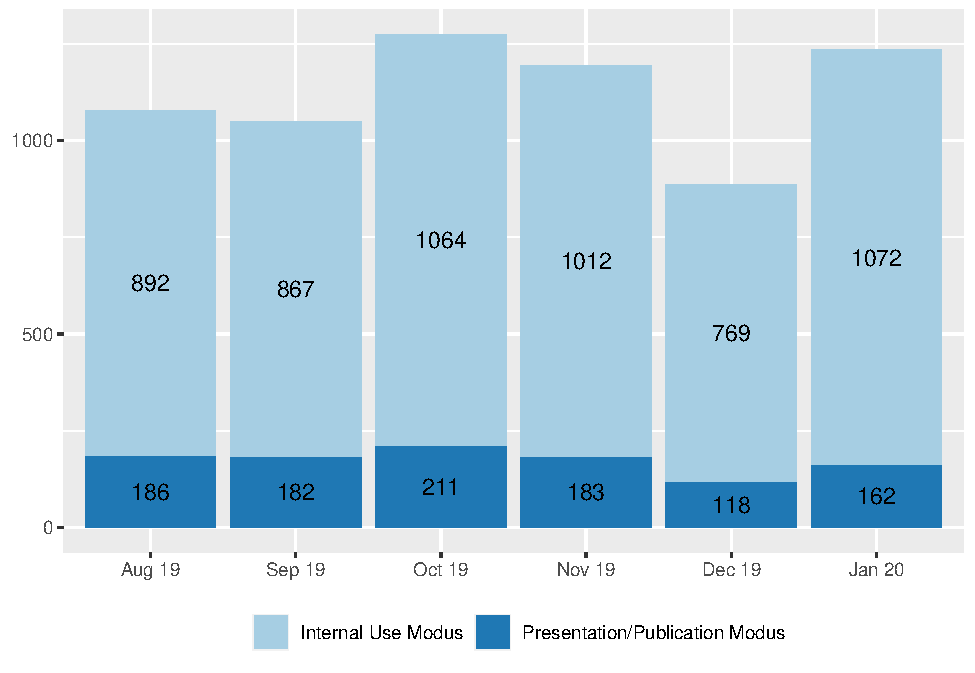
\includegraphics{./figures/iabfigure1.pdf}
\caption{\label{fig:iabfig1}Number of jobs via JoSuA}
\end{figure}

Some of the data products offered by the RDC-IAB\index{Research Data Center at the Institute for Employment Research} can also be downloaded as SUF\index{Scientific Use File} and used within the premises of the requesting institution. Anonymization for these data must be stronger than in the weakly anonymous\index{weakly anonymous} versions. The research data are stored in the Stata\index{Stata} file format and can be downloaded from a secure download platform after signing the DUA\index{data use agreement}. Details about storage and data use are specified in a data security concept that becomes part of the DUA. In this concept, the requesting institution declares that it will ensure suitable technical and organizational measures when dealing with de-facto anonymized\index{de-facto anonymized} data in compliance with data protection legislation. These measures include not sharing the data, restricting access to authorized personnel, ensuring sufficient security, using secure servers, and protecting hard drives against theft using modern encryption standards and deleting data securely at the end of the project period. Demand for SUF has been decreasing relative to weakly anonymized data products in recent years, partly driven by the improvements in access to both on-site\index{On-site} and remote execution\index{remote execution}. Downloading and storing SUF\index{Scientific Use File} outside of Germany is possible as long as the other ``safes'' are adhered to.

\hypertarget{safe-data}{%
\subsection{Safe Data}\label{safe-data}}

The data products provided by the RDC-IAB\index{Research Data Center at the Institute for Employment Research} are specifically created for the purpose of allowing external researchers access to the data. Before being customized by the RDC-IAB, these source data already undergo extensive preparation by the BA\index{BA}, the IAB\index{Institute for Employment Research}, or the partner institutes.\footnote{See section Making Data Usable for Research.} Still additional steps have to be taken before the data products can be accessed by external researchers. The sensitivity of RDC-IAB data products depends on the chosen access mode.

For \emph{weakly anonymous\index{weakly anonymous}} data, the data processing steps include the following:

\begin{itemize}
\tightlist
\item
  Drawing samples (administrative data, not surveys)
\item
  Pseudonymization\index{pseudonymization}\footnote{The source data used by the RDC-IAB are already pseudonymous.}
\item
  Coarsening of highly sensitive information (e.g., exact date of birth, residential community)
\item
  Omission of highly sensitive information that cannot be coarsened (e.g., disability status)
\item
  Providing higher levels of coarsening as a standard and only allowing lower levels in justified cases (e.g., 3-digit industry codes instead of 5-digit, federal state instead of district)
\end{itemize}

For \emph{de-facto anonymous\index{de-facto anonymized}} \emph{data}, additional data processing steps are as follows:

\begin{itemize}
\tightlist
\item
  Checking whether certain characteristics that might be used for re-identification show rare values
\item
  Additional coarsening and/or censoring
\item
  Omission of broader categories of data (e.g., omission of detailed establishment information in individual worker data sets)
\end{itemize}

These additional steps further reduce the disclosure risk for the data product and therefore enable data access via SUF\index{Scientific Use File}. The increased safety for the research data is traded against weaker requirements for safe settings. As a result, the research data can now be stored outside the RDC-IAB\index{Research Data Center at the Institute for Employment Research} secure computing environments while the portfolio of data security measures still ensures data protection.

Creating safe data for external data users is one of the main tasks of the RDC-IAB\index{Research Data Center at the Institute for Employment Research}, and it is done with the users explicitly in mind. Data products are still standardized and not produced on demand. Depending on the data product, updates are performed annually, biennially, or irregularly. In case of linked data products, the linkage is done during data generation since users are not allowed to perform further linkage at a later stage (except for the linkage of aggregate statistics). Fake test data are produced for most data products that can only be accessed on-site\index{On-site} or via remote execution\index{remote execution} so that users can prepare and test their code efficiently \citep{jacobebbinghaus2010}. These test data, however, do not meet the standards of a high-quality synthetic data product, and they should exclusively be used for code preparation.

Data are not only sampled, prepared, anonymized, and quality checked but also labelled and documented.\footnote{See section Making Data Usable for Research.} Data reports seek a good balance between accuracy and comprehensibility. They must convey important aspects about data origin and quality without drowning researchers in too much technical detail.

Total costs for the preparation of these data products are hard to measure because of several steps performed before the data are transferred to the RDC-IAB\index{Research Data Center at the Institute for Employment Research}. The final step of making the standardized data accessible, including data preparation, anonymization, documentation, and test data preparation, usually requires between fifteen and sixty fulltime-equivalent working days per data set. These numbers already take into account that some data sets build upon each other, so that complementary effects can be exploited. New data products, however, need more time and they are usually developed as parts of third-party funded research projects. Continuation or updates of those new data products then depends on follow-up funding or compatibility with the regular data production cycle of the RDC-IAB core staff.

Producing safe data for access outside the RDC-IAB\index{Research Data Center at the Institute for Employment Research} safe room is complicated by the current legal assessment prohibiting on-site\index{On-site} access to weakly anonymous\index{weakly anonymous} data outside the EU, even using the technical solutions outlined above.\footnote{See sections Making Data Usable for Researchers and Safe Settings.} This means that a choice had to be made between keeping analytic potential as high as possible and offering equal data access from all data access points\index{data access points}. In the end, a decision was reached that the safe data concept for data access within the EU would not be changed and that additional processing of the data would be conducted when users request access to the data from non-EU data access points. To mitigate limitations in the analytical potential for research data outside the EU, additional data processing steps are individually agreed upon together with the data users before the project starts. Since the RDC-in-RDC\index{Research-Data-Center in Research-Data-Center} project showed that international users often requested similar information for their research purposes, a modularized data anonymization concept was developed for all major data products to facilitate this coordination of the final anonymization strategy. This means that the process of coordination at the beginning of the project takes more time and that research teams sometimes must make tough decisions to make their projects feasible.

Since the RDC-IAB\index{Research Data Center at the Institute for Employment Research} only provides standardized data products, it cannot serve more individual project needs like special samples, additional and more detailed variables, or special linkages. While an alternative, fee-based data access mode for social data exists, this mode is not operated by the RDC-IAB and it is only available for German institutions. For international researchers, cooperation with the IAB\index{Institute for Employment Research} or another German research institution might prove to be the only way to conduct such research projects.

\hypertarget{safe-outputs}{%
\subsection{Safe Outputs}\label{safe-outputs}}

The way safe output is ensured at the RDC-IAB\index{Research Data Center at the Institute for Employment Research} depends on the data access mode for the research project. For SUF\index{Scientific Use File}, the responsibility to ensure safe output rests entirely with the requesting institution and the data users. The institution is mandated to refrain from any action that might compromise the anonymity of the statistical information contained in the data and is required to instruct data users accordingly. Thus, no statistical output that is not sufficiently anonymized is allowed to be published. The institutions can find assistance on what is meant by secure output in BA\index{BA} guidelines \citep{statistikderbundesagenturfurarbeit2018} or ask the RDC-IAB for assistance.

When data are used on-site\index{On-site} or via remote execution\index{remote execution}, both the RDC-IAB\index{Research Data Center at the Institute for Employment Research} and data users work together to ensure there is no re-identification of the data. The goal is that only completely anonymous (non-sensitive) results leave the safe computing environment. As a first step, data users are urged to keep their research output clean, clear, comprehensible, and well documented according to RDC-IAB guidelines. These guidelines describe in detail how program code has to be set up (including templates), what kind of documentation is needed, and in what file format output must be stored (usually as Stata log files and graphs but with some exceptions). Data users should also restrict their output to what is necessary and ensure that output can be exported without compromising anonymity or being rendered useless after the necessary SDC\index{SDC}. These preparations should be made during on-site visits or in IU-mode to reduce the amount of manual SDC required by RDC-IAB staff. The rules for documentation also require that all output considered for export must be generated from a script started by a single master file in the remote execution\index{remote execution}. This procedure ensures that all output is reproducible and all steps documented.

As a second step, the RDC-IAB\index{Research Data Center at the Institute for Employment Research} has developed a list of relatively simple rules that statistical output must satisfy. These rules might be overcautious in some cases but ensure that SDC\index{SDC} can be done quickly without having to consider all eventualities. The most important pillars of these rules are as follows:

\begin{itemize}
\tightlist
\item
  There is no disclosure of information based on one single observational unit (e.g., individual, household, or establishment). Every result must be based on at least twenty observational units. Primary cell suppression is used in tables that do meet this criterion.
\item
  Secondary cell suppression is used, which prevents the identification of information via subtotals and/or marginal totals. Secondary cell suppression might also be necessary in linked tables.
\end{itemize}

RDC-IAB\index{Research Data Center at the Institute for Employment Research} has developed some automated cell suppression routines that automatically pre-scan all output.\footnote{The script is based on Perl and was written by a staff member. It runs independently within JoSuA.} These routines are used both for the IU-mode and the PP-mode output\footnote{See section Safe Settings.} and reduce the amount of time needed for manual SDC\index{SDC} considerably. These routines, however, cannot account for all eventualities found in users output files, so the manual SDC by RDC-IAB\index{Research Data Center at the Institute for Employment Research} staff is still needed before output can be released. Excessive production of output or cases where manual SDC would become too time consuming are discussed bilaterally with the data users to find solutions that are easier to review and still satisfy the needs of the data users.

As a third step, rules for safe output are incorporated into the DUA\index{data use agreement}. The agreement commits data users to review their approved output to make sure inferences on single observational units are impossible. In case of any suspected violations, publication or transfer to third parties must be avoided until the case can be resolved with the assistance of the RDC-IAB\index{Research Data Center at the Institute for Employment Research} and the Legal Department of the IAB\index{Institute for Employment Research}. All approved results are documented and archived via the JoSuA\index{Job Submission Application} software.

Rules for on-site\index{On-site} data access or remote execution\index{remote execution} are equal for all on-site locations as well as users from within and outside of Germany. Therefore, rules for safe output were not changed as a result of the RDC-in-RDC\index{Research-Data-Center in Research-Data-Center} project.

\hypertarget{data-life-cycle-and-replicability}{%
\section{Data Life Cycle and Replicability}\label{data-life-cycle-and-replicability}}

\hypertarget{preservation-and-reproducibility-of-researcher-accessible-files}{%
\subsection{Preservation and Reproducibility of Researcher-Accessible Files}\label{preservation-and-reproducibility-of-researcher-accessible-files}}

RDC-IAB\index{Research Data Center at the Institute for Employment Research} versions, curates, and archives all its data products and older data products are currently not deleted. The IAB\index{Institute for Employment Research} department of Data and IT-Management curates IAB source data. Preliminary data management and sampling is done at the RDC-IAB using SAS\index{SAS}. Most final data refinement are performed using Stata\index{Stata}. RDC-IAB preserves all master files to enable the traceability and reproducibility of each data product.

RDC-IAB\index{Research Data Center at the Institute for Employment Research} provides the latest available data version to users. Older, archived versions of data sets are only available for the purpose of replication studies, or in exceptional cases, if the request is duly substantiated. It is also possible to change to the latest updated version during an ongoing research project.

\hypertarget{preservation-and-reproducibility-of-researcher-generated-files}{%
\subsection{Preservation and Reproducibility of Researcher-Generated Files}\label{preservation-and-reproducibility-of-researcher-generated-files}}

All research results generated at the RDC-IAB\index{Research Data Center at the Institute for Employment Research}, both on-site\index{On-site} or via remote execution\index{remote execution} can by restored as long as users follow the RDC-IAB guidelines and program their code accordingly. Not following those guidelines will often lead to code termination so that users have an interest in keeping their code error-free and well-structured. Each remote execution job in JoSuA\index{Job Submission Application} is started from a master file, which opens all underlying analysis code and sub-routines. At the end of each on-site use, researchers need to follow the same procedure in JoSuA to obtain code and results. It is not possible to get intermediate code versions or results without using JoSuA. The RDC-IAB preserves user generated code and original data for ten years. Only the original data have a persistent digital identifier. Users can also export and store their code from JoSuA after a manual check by RDC-IAB staff. RDC-IAB does not store intermediate data generated during a user project but such data should be reproducible using the preserved code. Access to user generated files or output is only possible with the permission of the original researchers and a DUA\index{data use agreement}. In case of misconduct or perceived misconduct, the IAB\index{Institute for Employment Research} follows its \href{https://www.iab.de/en/daten/replikationen.aspx}{procedure} for good scientific practice for data access and code.\footnote{Accessed on 06-15-2020}

\hypertarget{sustainability-and-continued-success}{%
\section{Sustainability and Continued Success}\label{sustainability-and-continued-success}}

\hypertarget{outreach}{%
\subsection{Outreach}\label{outreach}}

The RDC-IAB\index{Research Data Center at the Institute for Employment Research} uses different channels to inform interested researchers about the data products and data access possibilities. Most importantly, extensive information is available online at the RDC-IAB \href{https://fdz.iab.de/en.aspx}{website}.\footnote{Accessed on 06-15-2020} Additionally, the RDC-IAB newsletter keeps data users updated on news, such as new data sets or data updates. A continuous user survey helps to identifying any problems with the flow of information to the data users and adjustments can be made to the website. RDC-IAB staff presents data and data access options at conferences, workshops, and seminars. Users, RDC-IAB staff, and IAB\index{Institute for Employment Research} colleagues also present their research at national and international research conferences and publish in journals in various disciplines. These conference engagements often lead to questions or data requests from other researchers. International collaborations with high-ranking scholars boosted the interest in RDC-IAB data considerably \citep{card2015, schmieder2016}. The extension of data access points in Germany and abroad also exemplified the importance of word of mouth advertising. Quite often, users report their experiences with RDC-IAB data to their colleagues, leading to small clusters of researchers from the same institution working with the data.

RDC-IAB\index{Research Data Center at the Institute for Employment Research} is a partner in IDAN\index{International Data Access Network}. IDAN is a collaboration between six RDC\index{Research Data Center}s from France, Germany, the Netherlands, and the UK with the aim to enable working remotely with data from each partner at all partnering data access points\index{data access points}, thus facilitating access and enabling cross-country comparisons. This allows parallel (but separate) analysis for different countries. Appending data sets from different countries into a common database is legally forbidden and technically prevented. The \emph{Centre d'accès sécurisé aux données\index{Centre d'accès sécurisé aux données}} (CASD) in France and the RDC-IAB, for instance, have already prepared documentation to make researchers more aware of the possibilities for cross-country comparisons \citep{laible2020}. A joint conference in 2019 promoted the exchange between researchers, data providers, and stakeholders from different ministries in both countries and demonstrated the importance of access to administrative data and surveys.\footnote{For more information on IDAN, please visit \url{https://idan.network/} (Accessed on 06-15-2020).}

\hypertarget{revenue}{%
\subsection{Revenue}\label{revenue}}

There are no fees for RDC-IAB\index{Research Data Center at the Institute for Employment Research} data users, neither for data access nor for SDC\index{SDC} of research results. The RDC-IAB and its services are financed by a BA\index{BA} budget. This follows the recommendation of the RatSWD\index{RatSWD}, which is responsible for the accreditation of all German RDC\index{Research Data Center}s. Special mention should also be made of the free assistance provided by institutions that have a data access point\index{data access point} to RDC-IAB data.

The RDC-IAB\index{Research Data Center at the Institute for Employment Research} tries to finance projects for new data products through the acquisition of third-party funds. While third parties sometimes provided funding for generating new standardized data sets at the RDC-IAB\index{Research Data Center at the Institute for Employment Research}\footnote{One example is the data set ``Biographical Data of Social Insurance Agencies in Germany (BASiD)'' \citep{hochfellner2012}.}, today most funding is only available for genuine research projects and generating a new data set is a by-product of a larger research goal. Funding is sometimes available for infrastructure projects like the RDC-in-RDC\index{Research-Data-Center in Research-Data-Center} approach or Data without Boundaries\index{Data without Boundaries}.\footnote{Refer to the section Motivation and Background.}

Additional funding possibilities arise from linking survey data of collaborating institutions with the IAB\index{Institute for Employment Research}s administrative data (as long as consent to linkage was provided by the survey respondents). In 2011, the RDC-IAB\index{Research Data Center at the Institute for Employment Research} established the GRLC\index{German Record Linkage Center} in cooperation with the University of Duisburg-Essen to conduct research on record linkage and to provide services with record linkage applications \citep{antoni2019}. The implementation of the GRLC was funded by the German Research Foundation\index{German Research Foundation} (DFG) for three years. Today, the RDC-IAB\index{Research Data Center at the Institute for Employment Research} receives financial support from the collaborating institutes to perform the linkage, prepare and document the final linked data sets, and advise data users. One example of this kind of collaboration is the linked National Educational Panel Study\index{National Educational Panel Study} (NEPS) created with the Leibniz Institute for Educational Trajectories\index{Leibniz Institute for Educational Trajectories} (LIfBi).

\hypertarget{metrics-of-success}{%
\subsection{Metrics of Success}\label{metrics-of-success}}

The RDC-IAB\index{Research Data Center at the Institute for Employment Research} generates statistics to inform the IAB\index{Institute for Employment Research}, the BA\index{BA}, the RatSWD\index{RatSWD}, and researchers about data use at the RDC-IAB. These statistics reflect both the success of the data and the effort involved. The RDC-IAB provides statistics on active user projects, number of remote execution\index{remote execution} jobs, and on-site\index{On-site} uses each month/year online. A literature \href{https://fdz.iab.de/en/FDZ_Publications/FDZ_Literature_Database.aspx}{database} informs about papers based on RDC-IAB data.\footnote{Accessed on 06-15-2020} Not all data users, however, submit their papers to the RDC-IAB after the project ends, and data sets are not always cited correctly. Therefore, the actual number of papers using RDC-IAB\index{Research Data Center at the Institute for Employment Research} data is underestimated in this database. As a result, RDC-IAB measures its success by looking at the number of users and user projects rather than number of papers or citations.

As shown in Figure \ref{fig:iabfig2}, the numbers of users and user projects at the RDC-IAB continues to increase every year. In 2019, around 1,500 users worked in more than 700 projects.\footnote{In Figure 2, researchers who work in different projects are counted more than once.} The average duration of a research project is around three years. Bachelor theses or master theses usually do not take longer than six months.

\begin{figure}
\centering
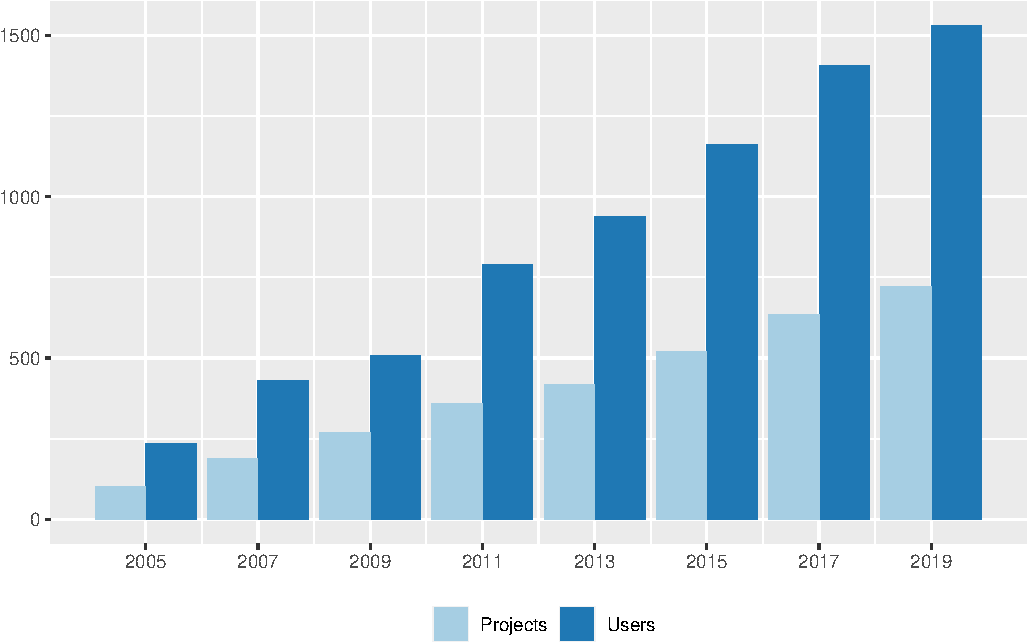
\includegraphics{figures/iabfig2-1.pdf}
\caption{\label{fig:iabfig2}Development of the number of users and number of projects at the RDC-IAB, 2005--2019}
\end{figure}

Since the implementation of the additional data access points\index{data access points}, the proportion of international users is constantly growing. Figure \ref{fig:iabfig3} shows the percentage share of contractual partners from Germany, the US, and other countries. While in 2012, less than 30 percent of all user projects were from a non-German facility, seven years later the value increased to 40 percent.

\begin{figure}
\centering
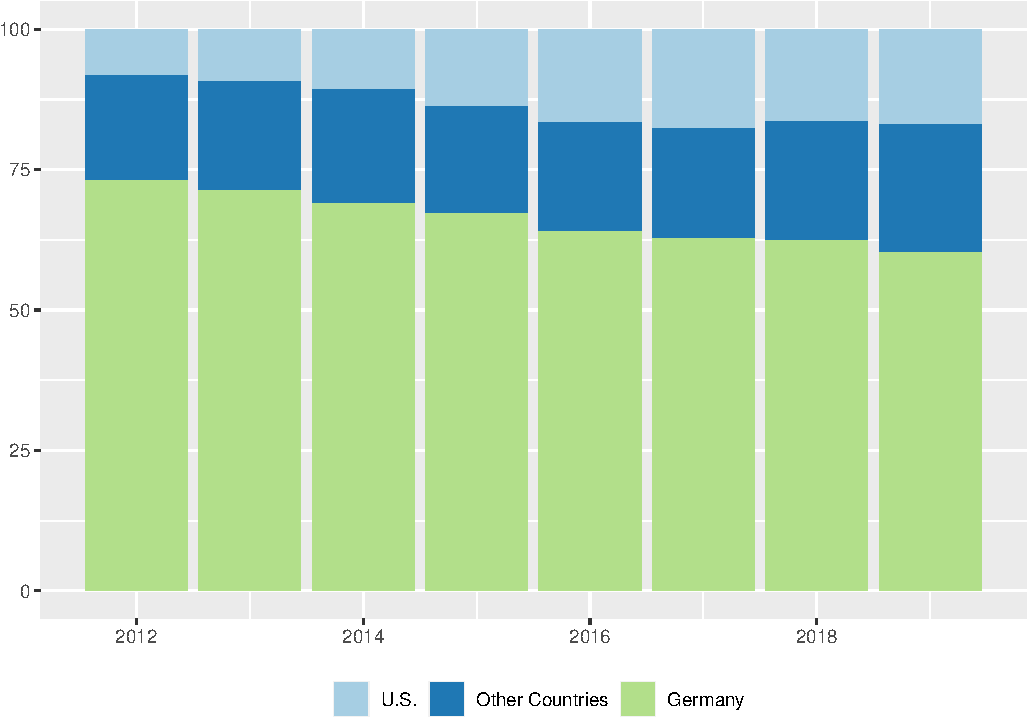
\includegraphics{figures/iabfig3-1.pdf}
\caption{\label{fig:iabfig3}Contractual partners of the RDC-IAB by country, 2012--2019}
\end{figure}

Additional statistics are also submitted to the annual activity report for all RDC\index{Research Data Center}s in Germany published by the RatSWD\index{RatSWD} {[}germandataforum2019{]}. Table \ref{tab:iabtable2} shows all publications with RDC-IAB\index{Research Data Center at the Institute for Employment Research} data in 2018, including publications from IAB\index{Institute for Employment Research} staff. There were 60 published papers in scientific journals in 2018, 45 of these in peer-reviewed journals. Additionally, 44 papers were published as working papers or reports and RDC-IAB data were used and cited in 41 books. As mentioned above, these numbers underestimate the true number of relevant publications in 2018.

\begin{table}

    \caption{\label{tab:iabtable2}Number of Publications in 2018, Including all Publications with RDC-IAB Data (Excluding Bachelor and Master Theses)}
    \centering
    \begin{tabular}[t]{lr}
    \toprule
    Publications & Numbers\\
    \midrule
    Papers & 60\\
    Thereof peer-reviewed papers & 45\\
    Books & 41\\
    Papers in anthologies & 8\\
    Grey literature (e.g., working papers, technical reports) & 14\\
    \bottomrule
    \end{tabular}
\end{table}

Apart from these general statistics, RDC-IAB\index{Research Data Center at the Institute for Employment Research} also gathers user feedback to learn what the users think about service quality, data documentation, data access modes, and additional user needs. At first, this was done using irregular user surveys \citep{wolter2018}, but currently two regular online user surveys are conducted. One survey focuses on service quality during the application phase. This survey is conducted shortly after the signing of the DUA\index{data use agreement} by the requesting institution. It is addressed to the researchers using the data, since they are usually more deeply involved in the application process than the representative providing the signature. The second survey covers user experiences after completed projects.

In general, user ratings are very good. For example, Figure \ref{fig:iabfig4} shows the ratings of data documentation and personal data advice. More than 90 percent of the survey respondent are satisfied (very good and good) with the data documentation. While 40 percent of all participants did not use personal data advice, nearly all others are satisfied. User suggestions, ideas, and critiques are essential to improve data access further to the extent possible given available resources.

\begin{figure}
\centering
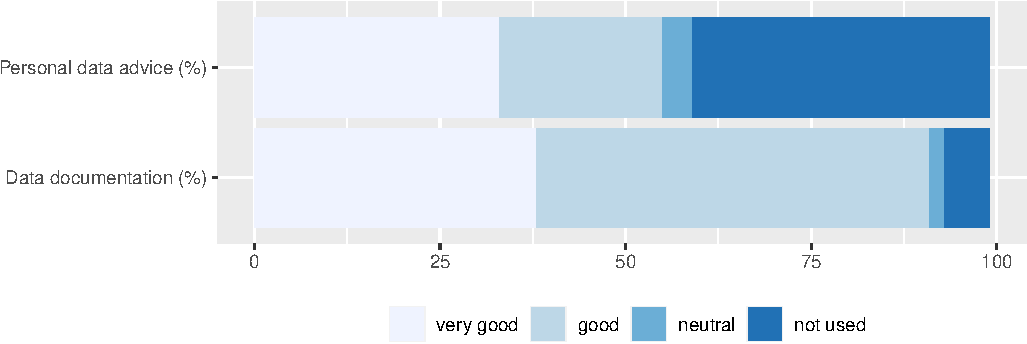
\includegraphics{figures/iabfig4-1.pdf}
\caption{\label{fig:iabfig4}User satisfaction with RDC-IAB services (options bad and very bad have not been chosen by respondents)}
\end{figure}

\hypertarget{about-the-authors-2}{%
\section*{About the Authors}\label{about-the-authors-2}}
\addcontentsline{toc}{section}{About the Authors}

\href{https://www.iab.de/en/ueberblick/mitarbeiter.aspx/Mitarbeiter/251}{Dana Müller} is the Head of the Research Data Center (RDC-IAB) of the Federal Employment Agency (BA) at the Institute for Employment Research (IAB) in Nuremberg, Germany. Previously, she was a researcher at the IAB and the Chemnitz University of Technology. In these positions, Dana Müller has worked with survey data, administrative data, and big-data; she has developed a deep knowledge and extensive experience in linkages of social security records, administrative information, and survey data. She has led many initiatives, including the project ``Quality of work and economic success'' and ``Biographical data of selected social insurance in Germany.'' Both projects were linking different administrative and survey data to advance social science research.

Dana has published several articles in leading social science journals and books. Her main research interests include sociology of the family and gender inequalities on the labor market, as well as linkage and confidentiality of administrative data. Her research on family and gender inequalities addresses repercussions of motherhood on labor market participation and discrimination as well as the influence of family-friendly arrangements in establishments on labor market behavior of mothers and fathers. Her work on research ethics addresses data confidentiality and methods of protecting privacy in the presence of an increasing demand of data in social sciences. She is IAB's representative at the \emph{Statistik Netzwerk Bayern} and elected member of the executive board of the DDI Alliance.

\href{https://www.iab.de/754/section.aspx/Mitarbeiter/72110}{Philipp vom Berge} is the Deputy Head of the Research Data Center (RDC-IAB) of the Federal Employment Agency (BA) at the Institute for Employment Research (IAB) in Nuremberg, Germany. He studied economics at the University of Regensburg, where he received his doctorate in 2013. Philipp has contributed to numerous IAB projects on data quality and data refinement. In recent years, his work on innovative research data focused on improving administrative labor market data and linked survey data to enhance their usability for minimum wage research.

Philipp's main research interest lies at the intersection of labor and regional economics. He has contributed to the emerging scientific literature on minimum wages in Germany and led several policy evaluation projects funded by the German government to accompany the introduction of the national statutory minimum wage. He has also worked on local spillovers, segregation, and policy evaluation using geocoded administrative research data.

\begin{invisible}
This is a workaround for citations in footnotes, please ignore.
@hochfellner2012
\end{invisible}

\putbib

